\chapter{The CLI-Tutor Tool}
% - Tool (CLI-Tutor)
%   - overview
%       - cirriculum
%       - lesson design
%            - deliberate emphasis on  easy vocabulary
%       - usability considerations
%       - safety considerations
%   - web version
%
\label{chap:clitutor}

\begin{figure}[htbp]
	\centering
	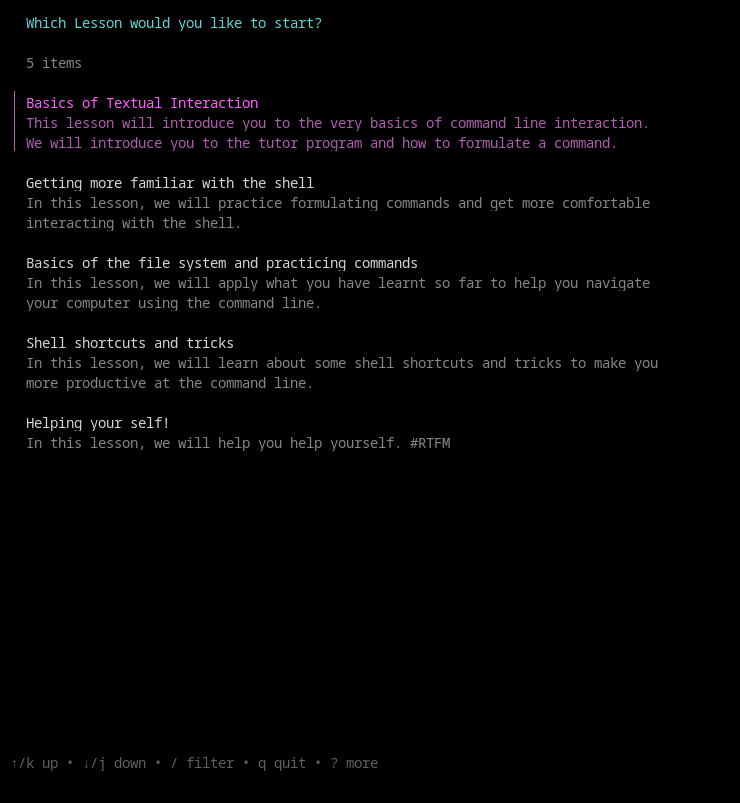
\includegraphics[width=0.8\textwidth]{img/climenu}
	\caption{Screen shot of \textit{CLI-Tutor} menu screen}
	\label{fig:clitutormenu}
\end{figure}

The \textit{CLI-Tutor} tool is a command line application written in the Go programming language. 


\section{Overview}
\subsection{Curriculum}
\subsection{Lesson Design}
\subsection{Usability Considerations}
\subsection{Safety Considerations}
\section{Web Version}


\begin{figure}[htbp]
	\centering
	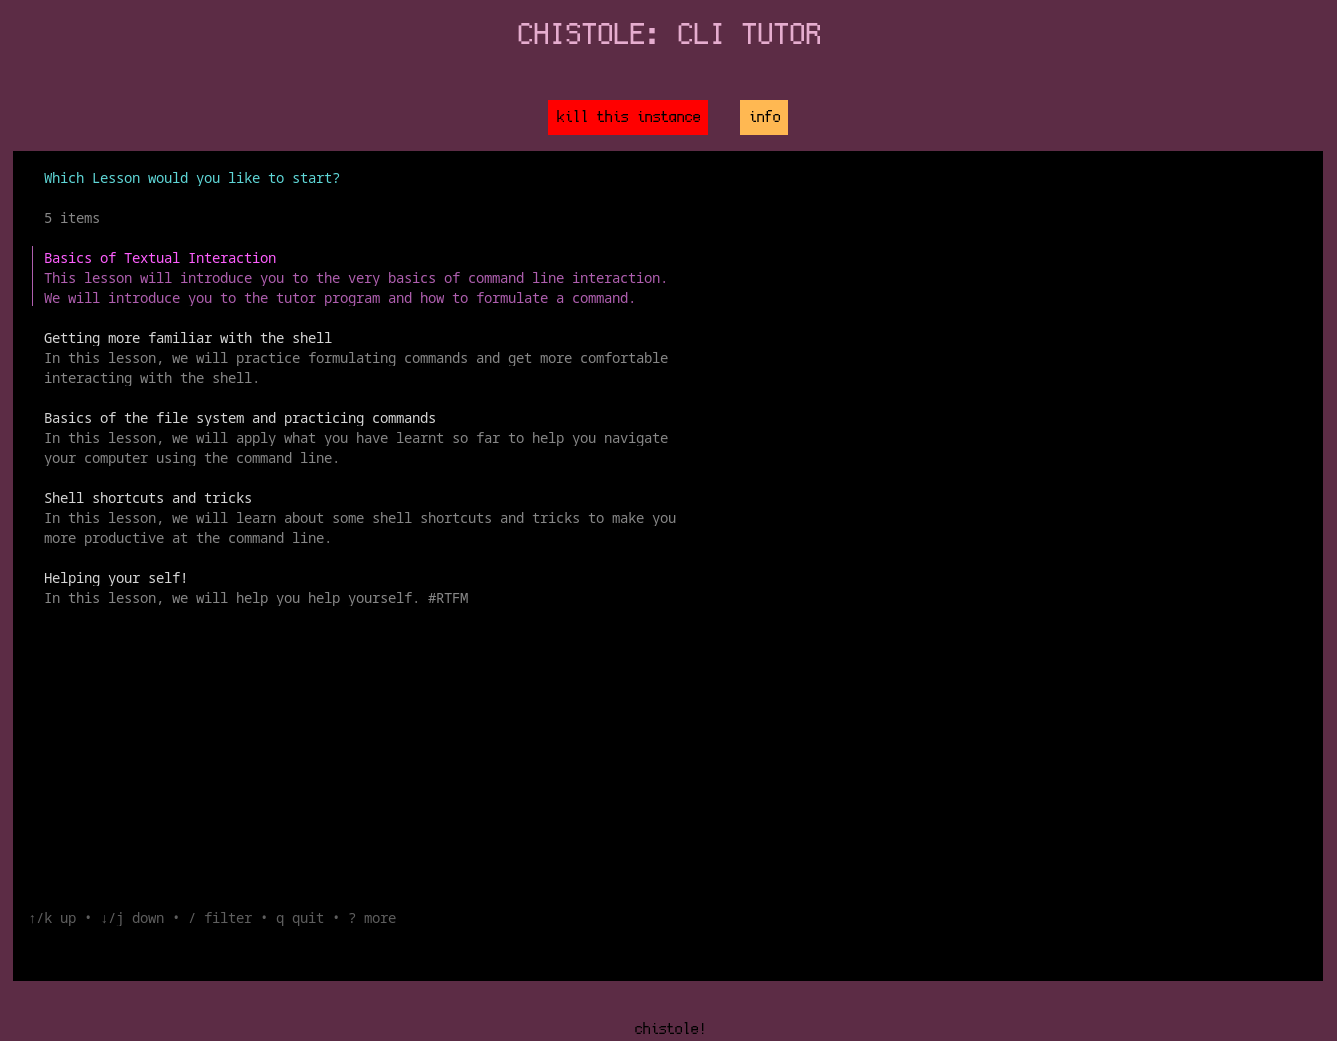
\includegraphics[width=1\textwidth]{img/cliwebfull}
	\caption{Screen shot of \textit{CLI-Tutor} menu screen in the web version.}
	\label{fig:webversion}
\end{figure}

\begin{figure}[htbp]
	\centering
	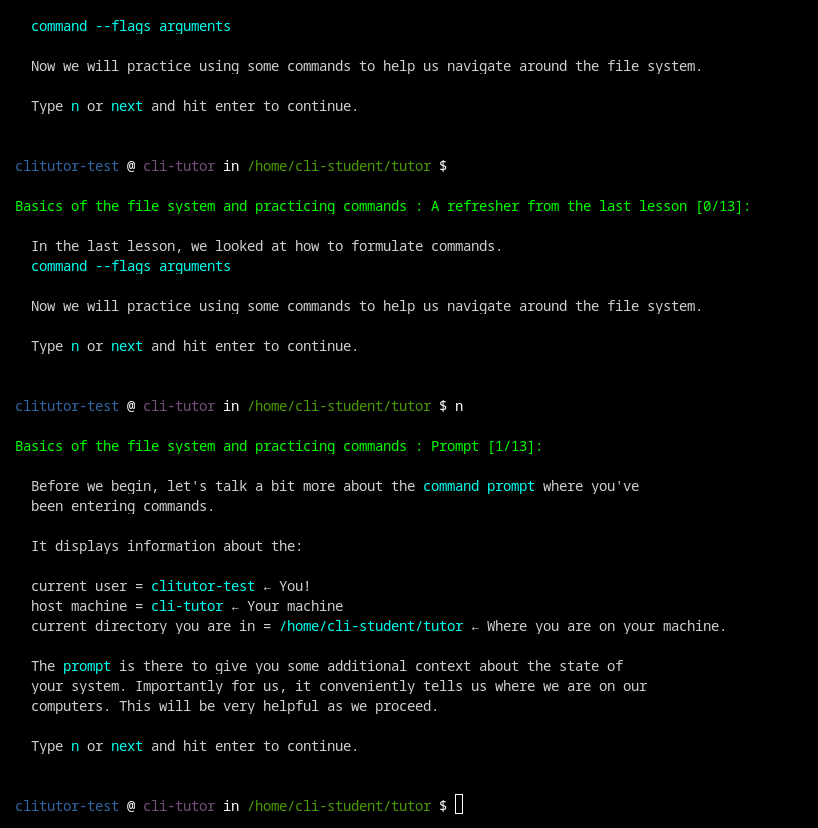
\includegraphics[width=1\textwidth]{img/cliexpansionfull}
	\caption{Screen shot of \textit{CLI-Tutor} menu screen in the web version.}
	\label{fig:webversion}
\end{figure}


